% ========================================
%	Header einbinden
% ========================================

\documentclass[bibtotoc,titlepage]{scrartcl}

% Deutsche Spracheinstellungen
\usepackage[ngerman,german]{babel, varioref}
\usepackage[T1]{fontenc}
\usepackage[utf8]{inputenc}

%\usepackage{marvosym}

\usepackage{amsfonts}
\usepackage{amssymb}
\usepackage{amsmath}
\usepackage{amscd}
\usepackage{amstext}

\usepackage{longtable}

%\usepackage{bibgerm}

\usepackage{footnpag}

\usepackage{ifthen}                 %%% package for conditionals in TeX
\usepackage[amssymb]{SIunits}
%Für textumflossene Bilder und Tablellen
%\usepackage{floatflt} - veraltet

%Für Testzwecke aktivieren, zeigt labels und refs im Text an.
%\usepackage{showkeys}

% Abstand zwischen zwei Absätzen nach DIN (1,5 Zeilen)
% \setlength{\parskip}{1.5ex plus0.5ex minus0.5ex}

% Einrückung am Anfang eines neuen Absatzes nach DIN (keine)
%\setlength{\parindent}{0pt}

% Ränder definieren
% \setlength{\oddsidemargin}{0.3cm}
% \setlength{\textwidth}{15.6cm}

% bessere Bildunterschriften
%\usepackage[center]{caption2}


% Problemlösungen beim Umgang mit Gleitumgebungen
\usepackage{float}

% Nummeriert bis zur Strukturstufe 3 (also <section>, <subsection> und <subsubsection>)
%\setcounter{secnumdepth}{3}

% Führt das Inhaltsverzeichnis bis zur Strukturstufe 3
%\setcounter{tocdepth}{3}
\usepackage[version=3]{mhchem}
	\mhchemoptions{minus-sidebearing-left=0.06em, minus-sidebearing-right=0.11em}
\usepackage{exscale}

\newenvironment{dsm} {\begin{displaymath}} {\end{displaymath}}
\newenvironment{vars} {\begin{center}\scriptsize} {\normalsize \end{center}}


\newcommand {\en} {\varepsilon_0}               % Epsilon-Null aus der Elektrodynamik
\newcommand {\lap} {\; \mathbf{\Delta}}         % Laplace-Operator
\newcommand {\R} { \mathbb{R} }                 % Menge der reellen Zahlen
\newcommand {\e} { \ \mathbf{e} }               % Eulersche Zahl
\renewcommand {\i} { \mathbf{i} }               % komplexe Zahl i
\newcommand {\N} { \mathbb{N} }                 % Menge der nat. Zahlen
\newcommand {\C} { \mathbb{C} }                 % Menge der kompl. Zahlen
\newcommand {\Z} { \mathbb{Z} }                 % Menge der kompl. Zahlen
\newcommand {\limi}[1]{\lim_{#1 \rightarrow \infty}} % Limes unendlich
\newcommand {\sumi}[1]{\sum_{#1=0}^\infty}
\newcommand {\rot} {\; \mathrm{rot} \,}         % Rotation
\newcommand {\grad} {\; \mathrm{grad} \,}       % Gradient
\newcommand {\dive} {\; \mathrm{div} \,}        % Divergenz
\newcommand {\dx} {\; \mathrm{d} }              % Differential d
\newcommand {\cotanh} {\; \mathrm{cotanh} \,}   %Cotangenshyperbolicus
\newcommand {\asinh} {\; \mathrm{areasinh} \,}  %Area-Sinus-Hyp.
\newcommand {\acosh} {\; \mathrm{areacosh} \,}  %Area-Cosinus-H.
\newcommand {\atanh} {\; \mathrm{areatanh} \,}  %Area Tangens-H.
\newcommand {\acoth} {\; \mathrm{areacoth} \,}  % Area-cotangens
\newcommand {\Sp} {\; \mathrm{Sp} \,}
\newcommand {\mbe} {\stackrel{\text{!}}{=}}     %Must Be Equal
\newcommand{\qed} { \hfill $\square$\\}
\renewcommand{\i} {\imath}
\def\captionsngerman{\def\figurename{\textbf{Abb.}}}

%%%%%%%%%%%%%%%%%%%%%%%%%%%%%%%%%%%%%%%%%%%%%%%%%%%%%%%%%%%%%%%%%%%%%%%%%%%%
% SWITCH FOR PDFLATEX or LATEX
%%%%%%%%%%%%%%%%%%%%%%%%%%%%%%%%%%%%%%%%%%%%%%%%%%%%%%%%%%%%%%%%%%%%%%%%%%%%
%%%
\ifx\pdfoutput\undefined %%%%%%%%%%%%%%%%%%%%%%%%%%%%%%%%%%%%%%%%% LATEX %%%
%%%
\usepackage[dvips]{graphicx}       %%% graphics for dvips
\DeclareGraphicsExtensions{.eps,.ps}   %%% standard extension for included graphics
\usepackage[ps2pdf]{thumbpdf}      %%% thumbnails for ps2pdf
\usepackage[ps2pdf,                %%% hyper-references for ps2pdf
bookmarks=true,%                   %%% generate bookmarks ...
bookmarksnumbered=true,%           %%% ... with numbers
hypertexnames=false,%              %%% needed for correct links to figures !!!
breaklinks=true,%                  %%% breaks lines, but links are very small
linkbordercolor={0 0 1},%          %%% blue frames around links
pdfborder={0 0 112.0}]{hyperref}%  %%% border-width of frames
%                                      will be multiplied with 0.009 by ps2pdf
%
\hypersetup{ pdfauthor   = {Hannes Franke; Julius Tilly},
pdftitle    = {V301 Innenwiderstand und Leistungsanpassung}, pdfsubject  = {Protokoll FP}, pdfkeywords = {V301, Innenwiderstand, Leistungsanpassung},
pdfcreator  = {LaTeX with hyperref package}, pdfproducer = {dvips
+ ps2pdf} }
%%%
\else %%%%%%%%%%%%%%%%%%%%%%%%%%%%%%%%%%%%%%%%%%%%%%%%%%%%%%%%%% PDFLATEX %%%
%%%
\usepackage[pdftex]{graphicx}      %%% graphics for pdfLaTeX
\DeclareGraphicsExtensions{.pdf}   %%% standard extension for included graphics
\usepackage[pdftex]{thumbpdf}      %%% thumbnails for pdflatex
\usepackage[pdftex,                %%% hyper-references for pdflatex
bookmarks=true,%                   %%% generate bookmarks ...
bookmarksnumbered=true,%           %%% ... with numbers
hypertexnames=false,%              %%% needed for correct links to figures !!!
breaklinks=true,%                  %%% break links if exceeding a single line
linkbordercolor={0 0 1},
linktocpage]{hyperref} %%% blue frames around links
%                                  %%% pdfborder={0 0 1} is the default
\hypersetup{
pdftitle    = {V301 Innenwiderstand und Leistungsanpassung}, 
pdfsubject  = {Protokoll AP}, 
pdfkeywords = {V301, Innenwiderstand, Leistungsanpassung},
pdfsubject  = {Protokoll AP},
pdfkeywords = {V301, Innenwiderstand, Leistungsanpassung}}
%                                  %%% pdfcreator, pdfproducer,
%                                      and CreationDate are automatically set
%                                      by pdflatex !!!
\pdfadjustspacing=1                %%% force LaTeX-like character spacing
\usepackage{epstopdf}
%
\fi %%%%%%%%%%%%%%%%%%%%%%%%%%%%%%%%%%%%%%%%%%%%%%%%%%% END OF CONDITION %%%
%%%%%%%%%%%%%%%%%%%%%%%%%%%%%%%%%%%%%%%%%%%%%%%%%%%%%%%%%%%%%%%%%%%%%%%%%%%%
% seitliche Tabellen und Abbildungen
%\usepackage{rotating}
\usepackage{ae}
\usepackage{
  array,
  booktabs,
  dcolumn
}
\makeatletter 
  \renewenvironment{figure}[1][] {% 
    \ifthenelse{\equal{#1}{}}{% 
      \@float{figure} 
    }{% 
      \@float{figure}[#1]% 
    }% 
    \centering 
  }{% 
    \end@float 
  } 
  \makeatother 


  \makeatletter 
  \renewenvironment{table}[1][] {% 
    \ifthenelse{\equal{#1}{}}{% 
      \@float{table} 
    }{% 
      \@float{table}[#1]% 
    }% 
    \centering 
  }{% 
    \end@float 
  } 
  \makeatother 
%\usepackage{listings}
%\lstloadlanguages{[Visual]Basic}
%\allowdisplaybreaks[1]
%\usepackage{hycap}
%\usepackage{fancyunits}

\usepackage{float}
\usepackage{caption}
\usepackage{wrapfig}
\usepackage{setspace}
\usepackage{threeparttable}
\usepackage{footnote}

\newfloat{formel}{htbp}{for}
\floatname{formel}{Formel}

% ========================================
%	Angaben für das Titelblatt
% ========================================

\title{Versuch 304 - Das Magnetische Moment\\				% Titel des Versuchs 
\large TU Dortmund, Fakultät Physik\\ 
\normalsize Anfänger-Praktikum}

\author{Jan Adam\\			% Name Praktikumspartner A
{\small \href{jan.adam@tu-dortmund.de}{jan.adam@tu-dortmund.de}}	% Erzeugt interaktiven einen Link
\and						% um einen weiteren Author hinzuzfügen
Dimitrios Skodras\\					% Name Praktikumspartner B
{\small \href{dimitrios.skodras@tu-dortmund.de}{dimitrios.skodras@tu-dortmund.de}}		% Erzeugt interaktiven einen Link
}
\date{18.Dezember 2012}				% Das Datum der Versuchsdurchführung

% ========================================
%	Das Dokument beginnt
% ========================================

\begin{document}

% ========================================
%	Titelblatt erzeugen
% ========================================

\maketitle					% Jetzt wird die Titelseite erzeugt
\thispagestyle{empty} 				% Weder Kopfzeile noch Fußzeile

% ========================================
%	Der Vorspann
% ========================================

%\newpage					% Wenn Verzeichnisse auf einer neuen Seite beginnen sollen
%\pagestyle{empty}				% Weder Kopf- noch Fußzeile für Verzeichnisse

\tableofcontents

%\newpage					% eine neue Seite
%\thispagestyle{empty}				% Weder Kopf- noch Fußzeile für Verzeichnisse
%\listoffigures					% Abbildungsverzeichnis

%\newpage					% eine neue Seite
%\thispagestyle{empty}				% Weder Kopf- noch Fußzeile für Verzeichnisse
%\listoftables					% Tabellenverzeichnis
\newpage					% eine neue Seite


% ========================================
%	Kapitel
% ========================================

%\section{Einleitung}				% Bei Bedarf

\section{Theorie}
Aus der Maxwell-Gleichung
\begin{equation}
\vec{\nabla} \cdot \vec{B} = 0
\end{equation}
 folgt direkt, dass es keine magnetischen Monopole gibt. Von der Komplexität her kommt  ein magnetischer Dipol einem Monopol am nächsten, dessen magnetisches Moment in diesem Versuch bestimmt werden soll.
 Der Dipol wird dazu in ein homogenes Magnetfeld eingeführt, wodurch ein Drehmoment auf ihn einwirkt, bis Dipol und Feldlinien des homogenen Magnetfeldes wieder gleichgerichtet sind.
 Ein homogenes Magnetfeld kann man durch ein sogenanntes Helmholz-Spulenpaares erzeugen. Es werden dazu zwei Spulen im Abstand $R$ voneinander aufgestellt. Dabei bezeichnet R den Radius der beiden Spulen. Werden nun beide Spulen gleichgerichtet von einem Gleichstrom durchflossen, so entsteht in ihrem Inneren durch Superposition der einzelnen Felder ein nahezu homogenes Magnetfeld.
  
\section{Aufbau}
Der im Versuch verwandte Dipol ist in eine kleine Vollkugel eingelassen. Die Kugel liegt in einer passenden Vertiefung, in der die Kugel nicht herumrollen kann. Von unten wird Luft eingeblasen, so dass die Kugel nahezu reibungsfrei auf dem Luftkissen schwebt.
Der gesamte Aufbau befindet sich im Inneren eines Helmholzspulenpaares, deren Radius jedoch nicht ganz dem Spulenabstand entspricht. Das Magnetfeld ist somit leicht inhomogen, da sich der Dipol jedoch sehr zentral auf der Symmetrieachse befindet kann dies vernachlässigt werden.
Das Magnetfeld der Spulen errechnet sich über das Biot-Savartsche Gesetzt
\begin{equation}
d \vec{B} = \frac{\mu_0 I}{4\pi} \frac{d \vec{s} \times \vec{r}}{r^3}
\end{equation} 
zu
\begin{equation}
B(0)=\frac{\mu_0 IR^2}{(R^2+x^2)^{3/2}}.
\end{equation}
Der Feldgradient $\frac{dB}{dx}$ entlang der Symmetrieachse errechnet sich entsprechend zu
\begin{equation}
\frac{dB}{dx} = -3\mu_0 IR^2 \frac{x}{(R^2+x^2)^{5/2}}.
\end{equation}
\section{Durchführung}
Das magnetische Moment des Dipols wird nun auf drei verschiedene Weisen berechnet.


\subsection{Gravitation}
In die Kugel mit dem Dipol wird ein etwa 20cm langer Stab gesteckt, an dem ein bewegliches Gewicht befestigt ist. Der Stab wird nun senkrecht zum Magnetfeld ausgerichtet, damit ihn einerseits ein Drehmoment durch die Gewichtskraft und andererseits ein Drehmoment durch das Magnetfeld wirkt. Beide Momente greifen die Kugel antiparallel an. Es wird nun so lange der Spulenstrom und dadurch auch das Magnetfeld erhöht, bis beide Drehmomente im Gleichgewicht liegen und der Stab ruht.
Im Gleichgewicht gilt:
\begin{equation}
\vec{\mu}_{Dipol} \times \vec{B} = m\cdot (\vec{r} \times \vec{g} ).
\end{equation}
Auf Grund der Winkelgleichheit lassen sich die Kreuzprodukte vereinfachen zu:
\begin{equation}
\mu_{Dipol} \cdot B = m\cdot r \cdot g.
\label{grav}
\end{equation}
Indem der Abstand der Masse zur Kugel variiert wird, kann die benötigte B-Feldstärke für verschiedene Drehmomente bestimmt werden. Eine lineare Ausgleichsrechnung mittels Gleichung \eqref{grav} bestimmt das magnetische Moment des Dipols.
\subsection{Harmonischer Oszillator}
Das durch das homogene B-Feld erzeugte Drehmoment ist eine rücktreibende Kraft. Entfernt man den zuvor angebrachten Stab und die Masse und lenkt die Kugel dann aus ihrer Ruhelage aus, so verhält sie sich wie ein harmonischer Oszillator und schwingt mit einer festen Frequenz hin und her.
Die Bewegung kann durch folgende Differentialgleichung beschrieben werden:
\begin{equation}
-|\vec{\mu}Dipol \times \vec{B}| = J_K \cdot \frac{d^2 \Theta}{dt^2}.
\end{equation}
Deren Lösung ist:
\begin{equation}
T^2=\frac{4\pi^2J_K}{\mu_{Dipol}} \frac{1}{B}
\label{oszi}
\end{equation}
Gemessen wird die Schwingungsdauer für verschiedene Magnetfeldstärken und durch lineare Ausgleichsrechnung wird mittels Gleichung \eqref{oszi} das magnetische Moment errechnet.
\subsection{Präzession}



\section{Auswertung}
\subsection{Fehlerrechnung}
Da viele für die Auswertung notwendigen Größen fehlerbehaftet sind, ist es wichtig, den Einfluss dieser Fehler auf die ermittelten
Größen herauszufinden. Neben den von den Messapparaturen verursachten Fehlern dienen der Mittelwert

\begin{formel}
\begin{equation}
 \bar{x} = \frac1N \sum_{i=1}^{N} x_i,
\end{equation}
\caption*{\small{$\bar{x}$ = Mittelwert, N = Anzahl der Messungen}}
\end{formel}

die Gaußsche Fehlerfortpflanzung

\begin{formel}
\begin{equation}
\Delta G = \sqrt{\sum_{i=1}^{N}\left( \frac{\partial G}{\partial x_i}\cdot \Delta x_i\right)^2},
\label{gauss}
\end{equation}
\caption*{$x_i$ = Variable, $\Delta x_i$ = Fehler der Variable}
\end{formel}

und die Standardabweichung des Mittelwerts

\begin{equation}
 \bar s = \sqrt{\frac{1}{N(N-1)} \sum_{i}^{N} (x_i - \bar{x})^2}.
\end{equation}

\subsection{Ermittlung der Apparaturkonstanten}
Für die Auswertung des Experiments sind einige, für die Apparatur individuellen Werte nötig. So die Daten des genutzten Helmholtz-Spulenpaars,
sowie der Billiardkugel. Sie wurden zu Versuchsbeginn aufgenommen. Der Fehler das Masse ergibt sich aus der kleinsten angezeigten Größenordnung
der zur Messung benutzten Waage. Der Fehler des Durchmessers wird von der Schieblehre abgelesen.

\begin{align*}
 d_H &= 0,138 \text{m} \\
 R_H &= 0,109 \text{m}\\
 N &= 195\\
 m_K &= 142,53 \text{g} \pm 0,01 \text{g}\\
 2r_K &= 53,65 \text{mm} \pm 0,05 \text{mm}
\end{align*}

Das Trägheitsmoment der Billiardkugel $J_K$ wird ermittelt und der Fehler nach \eqref{gauss} berechnet.

\begin{align}
\nonumber
 J_K &= \frac25 m_K r_K^2 \\
 &= 4,102 \cdot 10^{-5} \, \text{kgm}^2\\
 \nonumber
 \Delta J_K &= \sqrt{\left(\frac{\partial J_K}{\partial m_K} \Delta m_K \right)^2 + \left(\frac{\partial J_K}{\partial r_K} \Delta r_K \right)^2 } = J_K \sqrt{\left( \frac{\Delta m_K}{m_K} \right)^2 + \left( \frac{2 \, \Delta r_K}{r_K} \right)^2}\\
 &= 4,122 \cdot 10^{-9} \, \text{kgm}^2
\end{align}

\subsection[Ermittlung durch Ausnutzen der Gravitation]{Bestimmung des magnetischen Momentes eines Magnetens unter Ausnutzung der Gravitation}
Das von der Stromstärke $I$ erzeugte Magnetfeld $B(I)$ wirkt ein Drehmoment auf die kleine Masse $m_{kl}$ = 1,36 g zur Ausgleichung 
des vom Gravitationsfeld erzeugte Drehmoment.
\begin{table}[H]
 \begin{tabular}{c|c|c|c}
  i & $r$ in mm & $I$ in A & $B$ in mT\\
  \hline
1&	45,00&	1,62&	2,20\\
2&	50,00&	1,75&	2,37\\
3&	55,00&	1,85&	2,51\\
4&	60,00&	1,93&	2,62\\
5&	65,00&	2,10&	2,85\\
6&	70,00&	2,20&	2,98\\
7&	75,00&	2,30&	3,12\\
8&	80,00&	2,42&	3,28\\
9&	85,00&	2,51&	3,40\\
10&	90,85&	2,64&	3,58

 \end{tabular}
\caption{Magnetfeld $B$ in Abhängigkeit des Abstands $r$ der kleinen Masse}
\label{tabgrav}
\end{table}

Eine lineare Regression nach Gleichung \eqref{} durch GNUplot führt zu folgenden Parametern.

\begin{align}
\nonumber
B &= a \cdot r + b \intertext{mit} 
a &= (0,030 \pm 5,0 \cdot 10^{-4}) \, \frac{\text{mT}}{\text{mm}}\\
\nonumber
b &= (0,853 \pm 0,035) \, \text{mT}
\end{align}

\begin{figure}[H]
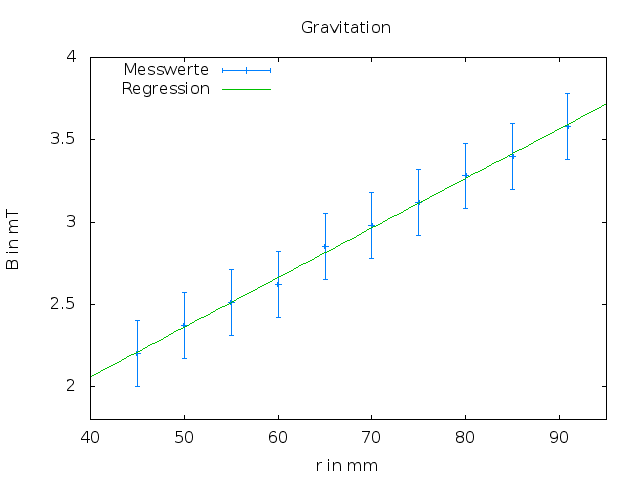
\includegraphics[width=0.8\textwidth] {pics/Gravitation.png}
\centering
\caption{lineare Abhängigkeit von $r$ und $B$}
\end{figure}

Nun lässt sich das magnetische Moment $\mu_{Grav}$ mitsamt Fehler angeben:

\begin{align}
 \nonumber
 \mu_{Grav} &= \frac{m_{kl}\,g}{a} \\
 &= 0,445\, \text{Am}^2\\
 \nonumber
 \Delta \mu_{Grav} &= \sqrt{\left(\frac{\partial \mu}{\partial m_{kl}}\Delta m_{kl} \right)^2 + \left(\frac{\partial \mu}{\partial a}\Delta a \right)^2} = \mu \sqrt{\left( \frac{\Delta m_{kl}}{m_{kl}}\right)^2 + \left( \frac{-\Delta a}{a}\right)^2}\\
 &= 5,0 \cdot 10^{-4}\, \text{Am}^2
\end{align}

\subsection[Ermittlung durch Schwingungsdauer]{Bestimmung des magnetischen Momentes über die Schwingungsdauer eines Magnetens}
Um größere Fehler durch Start-Stopp-Verzögerung zu vermeiden, wird über zehn Schwingungsperioden gemessen und das für jede Stromstärke
drei mal. 

 \begin{table}[H]
  \begin{tabular}{c|c|c|c|c|c|c|c}
i & $I$ in A & $^1T_{10}$ in s & $^2T_{10}$ in s & $^3T_{10}$ in s & $\bar T_{10}$ in s & $ 1/B$ in $1/$mT & $T^2$ in s$^2$\\
  \hline
1&	0,4&	25,72&	25,44&	25,72&	25,63&	1,844&	6,567\\
2&	0,8&	18,22&	18,25&	18,22&	18,23&	0,922&	3,323\\
3&	1,2&	15,13&	14,94&	15,00&	15,02&	0,615&	2,257\\
4&	1,6&	12,91&	12,90&	12,87&	12,89&	0,461&	1,662\\
5&	2,0&	11,50&	11,59&	11,50&	11,53&	0,369&	1,329\\
6&	2,4&	10,69&	10,59&	10,53&	10,60&	0,307&	1,124\\
7&	2,8&	9,81&	9,75&	9,81&	9,79&	0,263&	0,958\\
8&	3,2&	9,10&	9,13&	9,16&	9,13&	0,230&	0,834\\
9&	3,6&	8,62&	8,63&	8,69&	8,65&	0,205&	0,748\\
10&	4,0&	8,28&	8,22&	8,22&	8,24&	0,184&	0,679    
  \end{tabular}
\caption{Die Schwingungsdauer $T$ in Abhängigkeit der Stromstärke $I$}
  \label{tabschwing}
 \end{table}

Gleichung \eqref{} liefert die Abhängigkeit, die durch GNUplot mittels linearer Regression gefittet und mit folgenden Parametern 
beschrieben wird.

\begin{align}
\nonumber
T^2 &= c \cdot \frac1B + d \intertext{mit} 
c &= (3,554 \pm 0,012) \, \frac{\text{mT}}{\text{s}^2}\\
\nonumber
d &= (0,029 \pm 0,009) \, \text{s}^2
\end{align}

\begin{figure}[H]
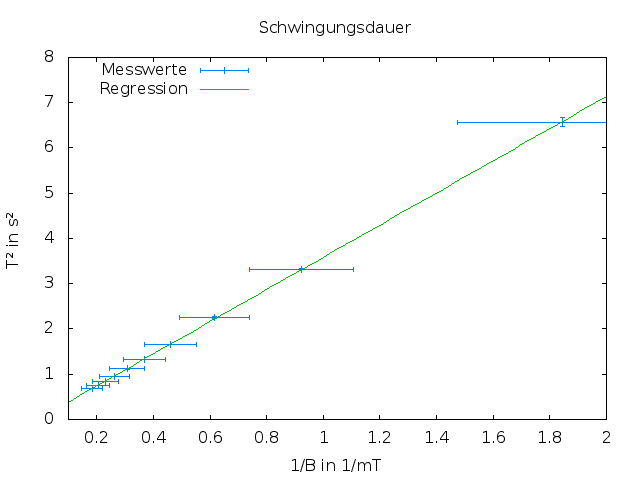
\includegraphics[width=0.8\textwidth] {pics/Schwingung.png}
\centering
\caption{lineare Abhängigkeit von $\frac{1}{B}$ und $T^2$}
\end{figure}

Das magnetische Moment $\mu_{Schw}$ wird nun mitsamt Fehler angeben:

\begin{align}
 \nonumber
 \mu_{Schw} &= \frac{4 \pi^2 J_{K}\,g}{c} \\
 &= 0,446\, \text{Am}^2\\
 \nonumber
 \Delta \mu_{Schw} &= \sqrt{\left(\frac{\partial \mu}{\partial J_{K}}\Delta J_{K} \right)^2 + \left(\frac{\partial \mu}{\partial c}\Delta c \right)^2} = \mu \sqrt{\left( \frac{\Delta J_{K}}{J_{K}}\right)^2 + \left( \frac{-\Delta c}{c}\right)^2}\\
 &= 0,012 \, \text{Am}^2
\end{align}

\subsection[Ermittlung durch Präzission]{Bestimmung des magnetischen Momentes über die Präzession eines Magneten}
Bei einer Stroboskopfrequenz $\nu_{Strob}$ von 4,5 Hz erschien der weiße Punkt am Stiel der Billiardkugel bei jedem Lichtimpuls
am gleichen Ort. Die vier markierten Werte in Tabelle \ref{tabpräz} entstehen durch Messen über zwei Präzessionsperioden, sodass hier nur
der halbierter Wert in den Mittelwert $\bar T_{p}$ einfließt.

 \begin{table}[H]
  \begin{tabular}{c|c|c|c|c|c|c|c}
i & $I$ in A & $^1T_{p}$ in s & $^2T_{p}$ in s & $^3T_{p}$ in s & $\bar T_{p}$ in s & $B$ in mT & $1/T$ in 1/s\\
  \hline
1&	0,4&	24,63&	24,78&	25,25&	24,89&	0,542&	0,040 \\
2&	0,8&	13,87&	13,53&	13,82&	13,74&	1,085&	0,073\\
3&	1,2&	9,38&	9,31&	9,16&	9,28&	1,627&	0,108\\
4&	1,6&	7,10&	7,41&	7,60&	7,37&	2,170&	0,136\\
5&	2,0&	5,97&	5,84&	5,88&	5,90&	2,712&	0,170\\
6&	2,4&	4,84&	5,25&	4,97&	5,02&	3,255&	0,199\\
7&	2,8&	\bf{7,94}&	4,32&	4,41&	4,23&	3,797&	0,236\\
8&	3,2&	\bf{7,53}&	3,75&	4,03&	3,85&	4,339&	0,260\\
9&	3,6&	\bf{6,85}&	3,47&	3,46&	3,45&	4,882&	0,290\\
10&	4,0&	\bf{6,09}&	3,09&	3,16&	3,10&	5,424&	0,323\\

  \end{tabular}
\caption{Die Präzessionsdauer $T$ in Abhängigkeit der Stromstärke $I$}
  \label{tabpräz}
 \end{table}

Aus Gleichung \eqref{} lassen sich durch GNUplot mittels linearer Ausgleichsrechnung die zur Bestimmung des magnetischen Moments $\mu$ 
nötigen Parameter bestimmen.

\begin{align}
\nonumber
\frac1T &= e \cdot B + f \intertext{mit} 
e &= (0,0576 \pm 5,79 \cdot 10^{-4}) \, \frac{1}{\text{mTs}}\\
\nonumber
f &= (0,0117 \pm 1,95 \cdot 10^{-3}) \, \frac{1}{\text{s}}
\end{align}

\begin{figure}[H]
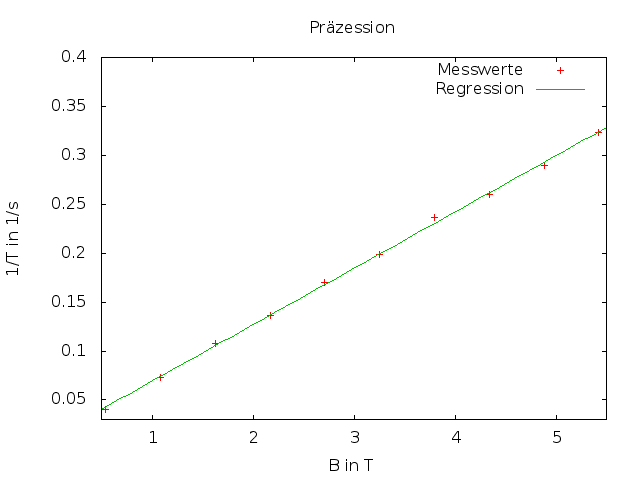
\includegraphics[width=0.8\textwidth] {pics/Praezession.png}
\centering
\caption{lineare Abhängigkeit von $\frac{1}{B}$ und $T^2$}
\end{figure}

Das magnetische Moment $\mu_{Praez}$ wird nun mitsamt Fehler angeben:

\begin{align}
 \nonumber
 \mu_{Praez} &= 4\pi^2 J_K \nu_{Strob} \cdot e \\
 &= 0,420\, \text{Am}^2\\
 \nonumber
 \Delta \mu_{Praez} &= \sqrt{\left(\frac{\partial \mu}{\partial J_{K}}\Delta J_{K} \right)^2 + \left(\frac{\partial \mu}{\partial e}\Delta e \right)^2} = \mu \sqrt{\left( \frac{\Delta J_{K}}{J_{K}}\right)^2 + \left( \frac{\Delta e}{e}\right)^2}\\
 &= 5,79 \cdot 10^{-4}\, \text{Am}^2
\end{align}

\section{Diskussion}
Übersichtlich zusammengestellt nochmal das magnetische Moment, errechnet aus drei verschiedenen Ansätzen.

\begin{align*}
 \mu_{Grav} &= 0,445 \pm 5,0 \cdot 10^{-4} \text{Am}^2\\
 \mu_{Schw} &= 0,446 \pm 1,2 \cdot 10^{-2} \text{Am}^2\\
 \mu_{Praez} &= 0,420 \pm 5,8 \cdot 10^{-4} \text{Am}^2\\
\end{align*}

Da bei keiner Methode der ermittelte Wert stark von den anderen beiden abweicht, ist davon auszugehen, dass der Wert des magnetischen 
Moments des Magneten inmitten der Billiardkugel sich in der Nähe von 0,44 Am$^2$ befindet. Schwierig beim Ansatz mit Ausnutzung der
Gravitation ist die nötige Genauigkeit der Apparatur zur Einstellung der Stromstärke. So ist es schwer möglich, die kleine Masse m$_{kl}$
zur Ruhe zu bringen. Des Weiteren gestaltet sich die Methode der Präzession als fehleranfällig, da die Synchonisation von Stroboskopfrequenz
und Drehfrequenz der Kugel nicht Restlos gelingt. Über eine Präzessionsrotation hinweg nimmt die Eigenrotation der Kugel sehr stark ab und bleibt nicht fest bei den 4,5Hz. Zudem war eine Nutation nicht restlos vermeidbar, was ebenfalls Einfluss auf das Ergebnis hat. 
Vermutlich wurde die Kugel um einen zu großen Winkel ausgelenkt, so dass eine Nutation begünstigt wurde. Die Betrachtung des Magneten als
harmonischen Oszillator verhilft vermutlich zum besten Ergebnis. Durch die Messung über 10 Schwingungsperioden und die leicht feststellbare Dauer
einer Periode, wodurch die Abweichungen der einzelnen Messungen untereinander sehr gering sind und dass die Kugel durch das Luftkissen fast garnicht abgebremst wird,
 ist diese Aussage berechtigt.


% ========================================
%	Literaturverzeichnis
% ========================================

%\bibliographystyle{plainnat}			% Bibliographie-Style auswählen
%\bibliography{BIBDATEI}			% Literaturverzeichnis

% ========================================
%	Das Dokument endent
% ========================================

\end{document}
